% ------------------------------------------------------------------------------
% Slides 4b-4d: Láminas Oficiales del Atlas - Evolución Temporal y Competencia de Picos
% ------------------------------------------------------------------------------

% Frame 1: Alta separabilidad inicial
\begin{frame}{Evidencia Experimental: Día de Alta Separabilidad - 2026-09-15}
    \centering
    \vskip -0.15cm
    {\scriptsize Habla natural inicial: apertura mandibular clara para /e/, sonrisa marcada en /i/ con baja interferencia de lengua.}\\[3pt]
    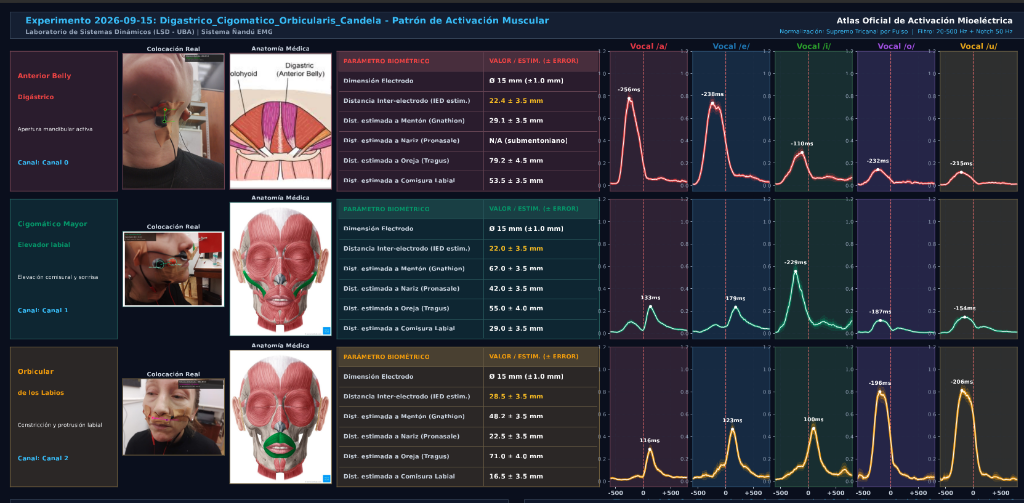
\includegraphics[width=\linewidth,height=0.76\textheight,keepaspectratio]{figuras/competencia_picos_02_dia_alta_separabilidad_0915.png}
\end{frame}

% Frame 2: Pérdida forzando vocales
\begin{frame}{Evidencia Experimental: Pérdida por Gesto Forzado - 2026-10-28}
    \centering
    \vskip -0.15cm
    {\scriptsize Tarea forzada (/i/ sonriendo, /a/ abriendo): el hablante usa más la lengua en /e/, alterando los picos de apertura.}\\[3pt]
    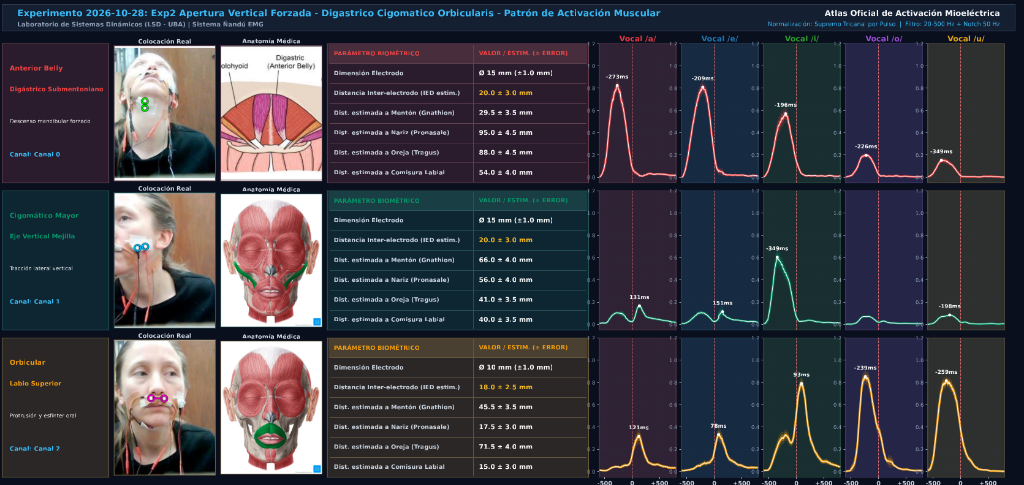
\includegraphics[width=\linewidth,height=0.76\textheight,keepaspectratio]{figuras/competencia_picos_01_dia_perdida_forzada_1028_exp2.png}
\end{frame}

% Frame 3: Pérdida en habla natural
\begin{frame}{Evidencia Experimental: Pérdida en Habla Natural - 2026-10-28}
    \centering
    \vskip -0.15cm
    {\scriptsize Desacople motriz: mayor reclutamiento de lengua tanto en /e/ como en /i/, produciendo choque de picos en mentón.}\\[3pt]
    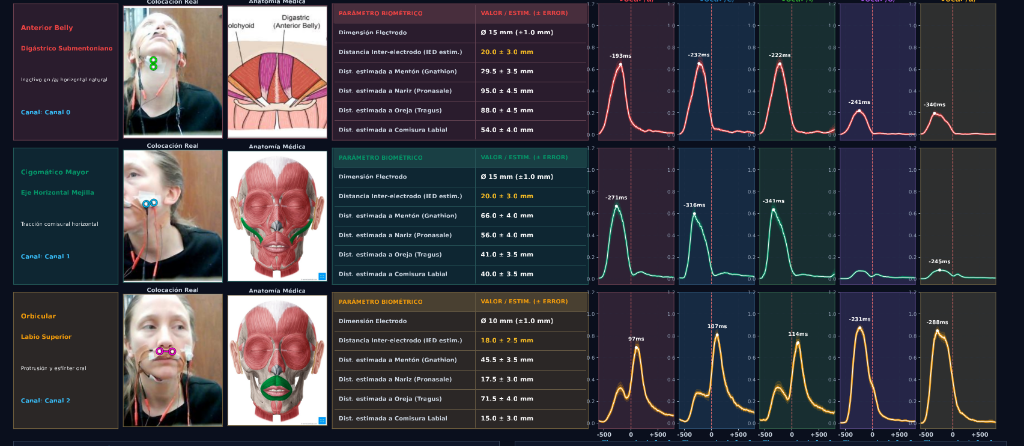
\includegraphics[width=\linewidth,height=0.76\textheight,keepaspectratio]{figuras/competencia_picos_03_dia_perdida_natural_1028_exp1.png}
\end{frame}
